\documentclass[12pt]{article}

\usepackage{graphicx}
\usepackage{xcolor}
\usepackage{hyperref}
\usepackage{float}
\usepackage{placeins}
\usepackage{subcaption}
\usepackage{geometry}

\geometry{margin=1in}

\hypersetup{
colorlinks=true,
urlcolor=blue,
}

\raggedbottom

\title{SSL-project Report}
\author{Jahnavi Alaparthi}

\begin{document}

\maketitle

% ======================================================
\section{External Libraries Used}

The following external libraries were used in the development of the Mini Game Hub project. These libraries helped in building a fully interactive, modular, and data-driven gaming system.

\begin{itemize}

\item \textbf{Pygame}:  
Pygame is the core library used for building the graphical interface of the project. It provides functionality for rendering game boards, drawing shapes (circles, grids), handling mouse clicks, and updating real-time game states. It is essential for creating interactive 2D games like TicTacToe, Connect4, and Othello.

\item \textbf{NumPy}:  
NumPy is used for efficient numerical computation and for representing game boards as matrices. It simplifies operations like checking win conditions, counting pieces, and updating board states quickly.

\item \textbf{Matplotlib}:  
Matplotlib is used to visualize game statistics such as number of wins per player and distribution of games played. It generates bar charts and pie charts which make data analysis visually understandable.

\item \textbf{sys}:  
The sys module is used for handling command-line arguments, which allows passing player names while running the program. It is also used for safe program exit using sys.exit().

\item \textbf{subprocess}:  
Subprocess is used to run external shell scripts like leaderboard.sh from within Python. This enables separation of logic between Python game engine and shell-based leaderboard computation.

\item \textbf{datetime}:  
This module is used to record the exact time and date of each game result. It helps in maintaining a proper history log of matches played.

\item \textbf{os}:  
The os module is used for file system operations such as checking if files exist, creating history files, and managing paths across different operating systems.

\item \textbf{collections.Counter}:  
Counter is used to efficiently count occurrences of players' wins and number of games played. It is highly useful for generating leaderboard statistics.

\item \textbf{csv}:  
The csv module is used to store and retrieve game history in a structured format. Each match result is stored as a row with winner, loser, game type, and timestamp.

\end{itemize}

\section{Design and Architecture}

The Mini Game Hub is designed as a modular, menu-driven gaming system built using Python. The architecture follows a centralized controller model where a single main file (\texttt{game.py}) manages the user interface, game selection, result tracking, and analytics, while individual games (such as TicTacToe, Connect4, and Othello) are implemented as separate modules.

\subsection{System Overview}

The system is structured into four major components:

\begin{itemize}
    \item \textbf{Main Controller (game.py):} Handles the graphical user interface (GUI), game flow control, player input, and navigation between screens.
    \item \textbf{Game Modules:} Independent Python modules for each game. Each module implements its own game logic and returns the result (winner or draw) to the main controller.
    \item \textbf{Data Storage:} A CSV-based system (\texttt{history.csv}) is used to store match results including winner, loser, date, and game type.
    \item \textbf{Analytics Module:} Uses Matplotlib to generate visual insights such as top players and game distribution.
\end{itemize}

\subsection{Architecture Design}

The system follows a layered architecture:

\begin{enumerate}
    \item \textbf{Presentation Layer:} Built using Pygame, responsible for rendering menus, buttons, background images, and post-game screens.
    \item \textbf{Control Layer:} Manages game transitions, user actions, and navigation between different screens such as main menu, game screens, and result screens.
    \item \textbf{Logic Layer:} Contains individual game logic modules that execute gameplay independently.
    \item \textbf{Data Layer:} Stores and retrieves game history using CSV files and processes it for analytics.
\end{enumerate}

\subsection{Key Design Features}

\begin{itemize}
    \item \textbf{Modularity:} Each game is implemented as a separate module, making the system easy to extend and maintain.
    \item \textbf{Event-Driven GUI:} The interface is built using Pygame event handling, allowing real-time interaction through buttons and mouse clicks.
    \item \textbf{Separation of Concerns:} Game logic, UI rendering, and data storage are clearly separated to improve maintainability.
    \item \textbf{Dynamic Visualization:} Player performance and game statistics are visualized using bar charts and pie charts.
    \item \textbf{Scalable Design:} New games can be added without modifying the core architecture, only requiring integration into the main controller.
\end{itemize}

\subsection{Workflow}

The workflow of the system is as follows:

\begin{enumerate}
    \item The user launches the application and enters player names.
    \item The main menu is displayed with available game options.
    \item On selecting a game, control is passed to the respective game module.
    \item The game executes independently and returns the result.
    \item The result is recorded in the CSV file.
    \item A post-game screen is displayed with options such as replay, graphs, and leaderboard.
    \item Users can view analytics or return to the main menu.
\end{enumerate}

\subsection{Conclusion}

The design of the Mini Game Hub ensures modularity, scalability, and ease of interaction. The separation of UI, game logic, and data processing allows the system to be extended with additional games and features without affecting existing functionality.
% ======================================================
\section{Features Implemented}

\begin{itemize}

\item Secure user authentication system with login validation.
\item Selection menu for multiple games.
\item Real-time graphical game interface using Pygame.
\item Modular design using object-oriented programming and inheritance.
\item Central leaderboard system for tracking performance.
\item Graphical visualization of statistics using Matplotlib.
\item Persistent storage using CSV and TSV files.
\item Smooth navigation between multiple game windows.
\item Input validation and error handling for robustness.

\end{itemize}

% ======================================================

\section{Project Structure Explanation}

\begin{verbatim}
SSL-PROJECT/
│
├── games/
├── game.py
├── leaderboard.sh
├── history.csv
├── users.tsv
├── main.sh
├── Makefile
├── README.md
│
└── report.pdf/
    ├── report.tex
    ├── references.bib
\end{verbatim}

\subsection{Description of Files and Folders}

\begin{itemize}
    \item \textbf{games/} -- Contains all individual game modules such as \texttt{tictactoe.py}, \texttt{connect4.py}, and \texttt{othello.py}. Each game runs independently and returns the result to the main controller.

    \item \textbf{game.py} -- The main controller of the project. It handles the GUI using Pygame, manages game selection, records results, and displays graphs and leaderboards.

    \item \textbf{leaderboard.sh} -- A shell script used to generate and sort leaderboard data based on wins, losses, ratio, or game type.

    \item \textbf{history.csv} -- Stores all match results including winner, loser, timestamp, and game type. Used for analytics and leaderboard generation.

    \item \textbf{users.tsv} -- Stores user information in a tab-separated format for tracking players.

    \item \textbf{main.sh} -- Shell script used to launch the project easily from terminal and manage execution flow.

    \item \textbf{Makefile} -- Automates project setup and execution commands for easier compilation and running.

    \item \textbf{README.md} -- Provides documentation about the project, setup instructions, and usage guidelines.

    \item \textbf{report.pdf/} -- Contains the project report files written in LaTeX format.

    \item \textbf{report.tex} -- Main LaTeX file used to generate the final project report.

    \item \textbf{references.bib} -- Bibliography file containing references used in the report.
\end{itemize}


% ======================================================
\section{Game Navigation Flow}

\begin{enumerate}

\item User logs in using authentication system.
\item Main menu is displayed using Pygame GUI.
\item User selects a game from available options.
\item Selected game runs in a separate window.
\item Game result is computed and displayed.
\item Result is stored in history.csv.
\item Leaderboard and graphs are generated after completion.
\item User can continue playing or exit.

\end{enumerate}

% ======================================================
\section{Usage}
\begin{figure}[htbp]
\centering
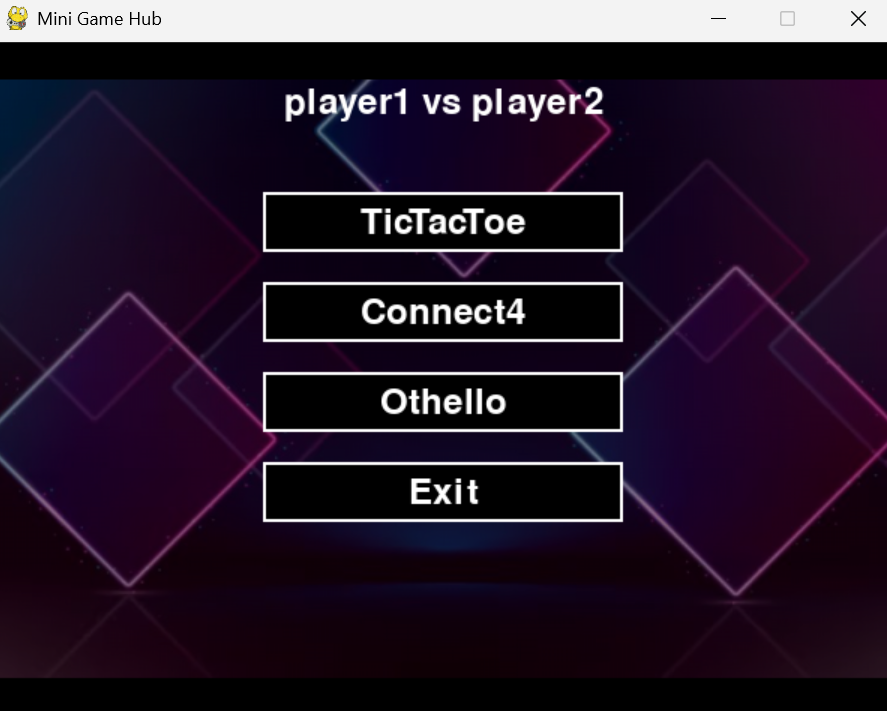
\includegraphics[width=0.8\textwidth]{mainwindow.png}
\caption{Game Interface}
\end{figure}

\begin{figure}[H]
\centering
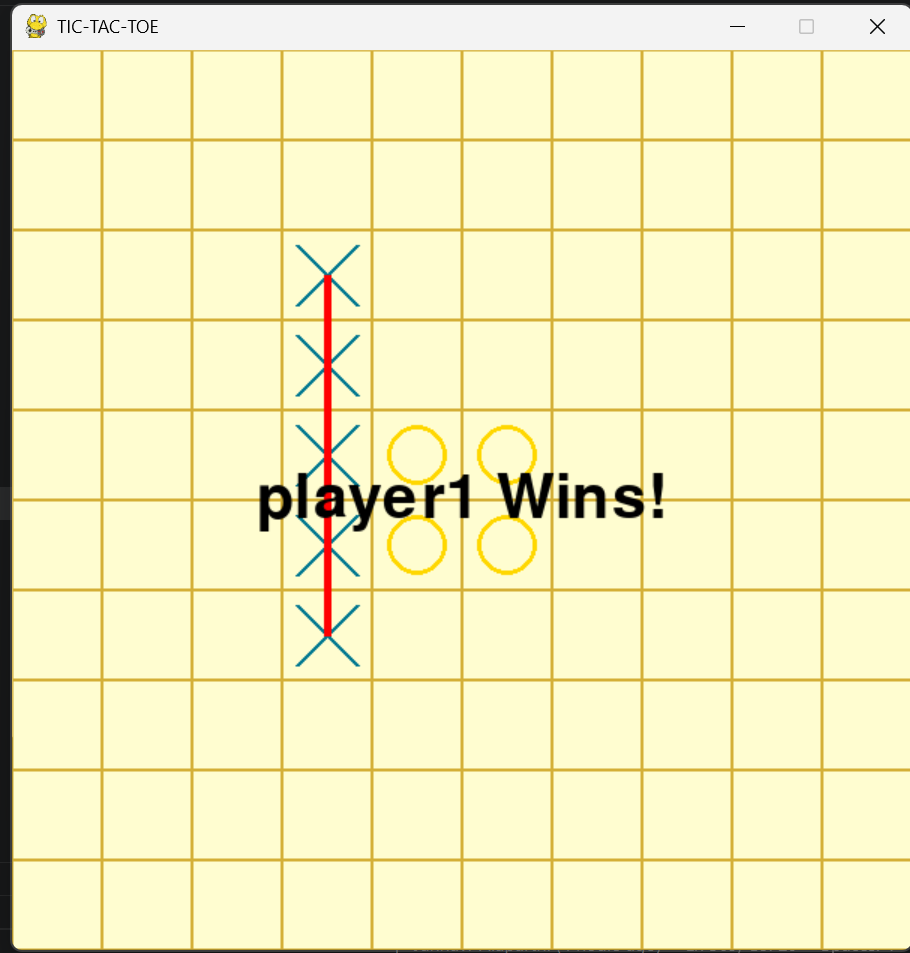
\includegraphics[width=0.8\textwidth]{tictactoe.png}
\caption{TicTacToe Gameplay}
\end{figure}

\begin{figure}[H]
\centering
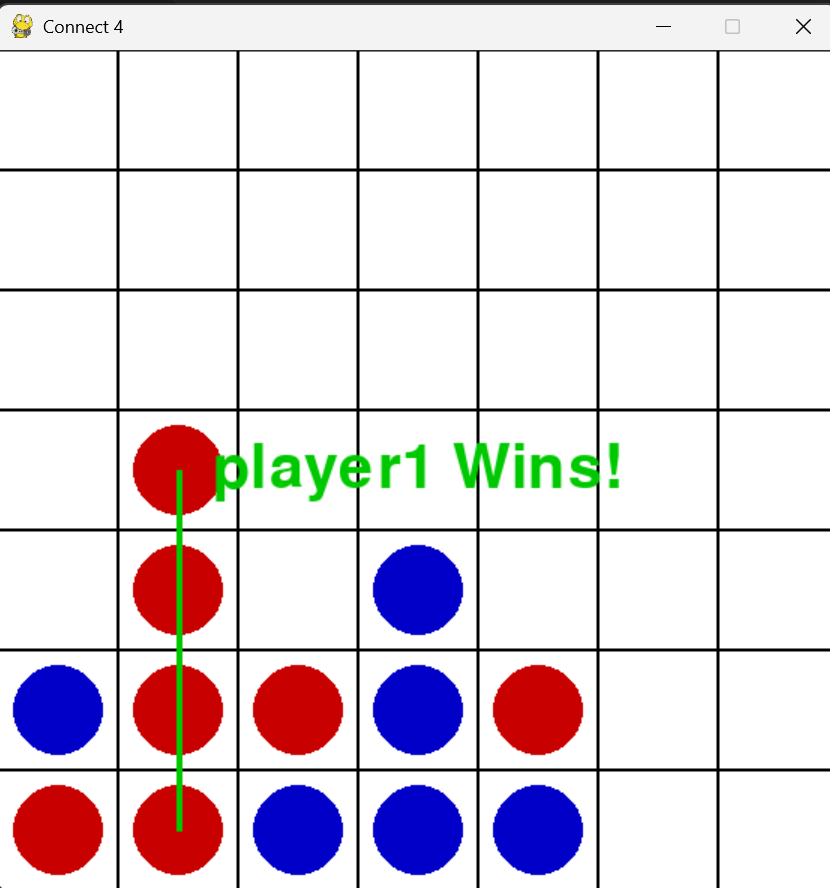
\includegraphics[width=0.8\textwidth]{connect4.png}
\caption{Connect4 Gameplay}
\end{figure}

\begin{figure}[H]
\centering
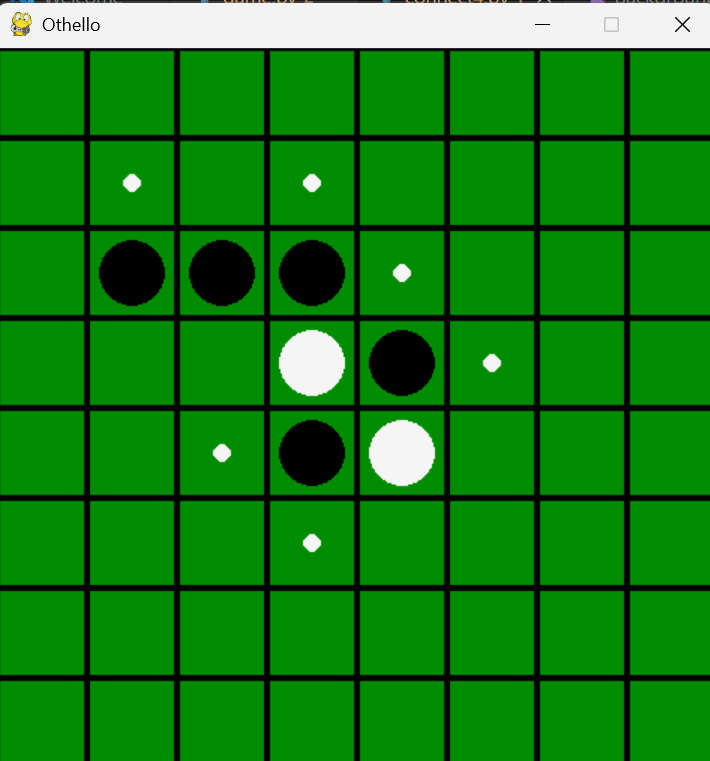
\includegraphics[width=0.8\textwidth]{othello.png}
\caption{Othello Gameplay}
\end{figure}

\begin{figure}[H]
\centering
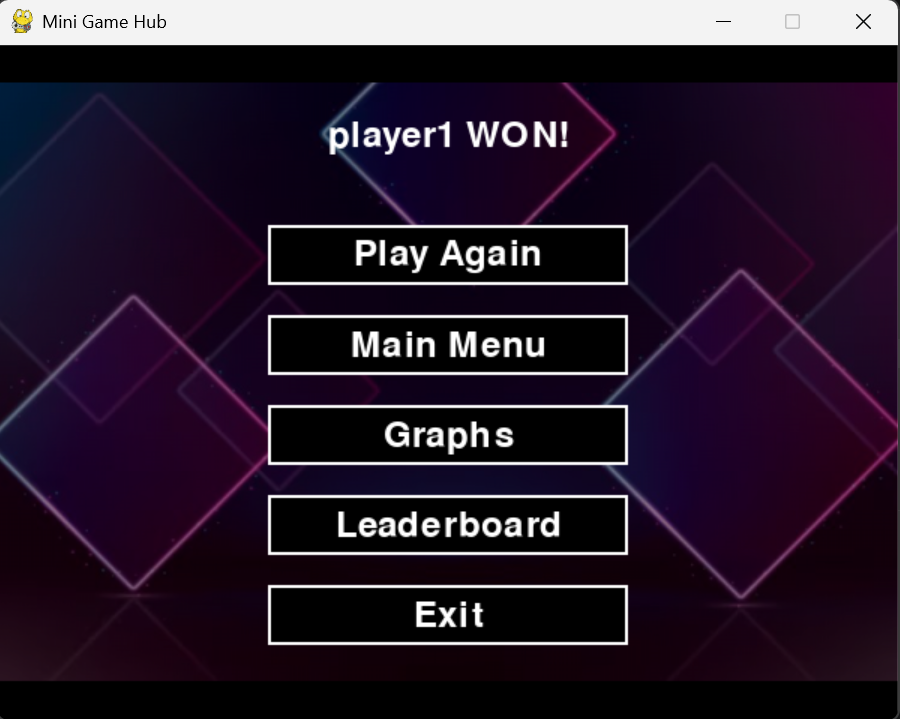
\includegraphics[width=0.8\textwidth]{after-game-window.png}
\caption{After game completed interface}
\end{figure}

\begin{figure}[H]
\centering
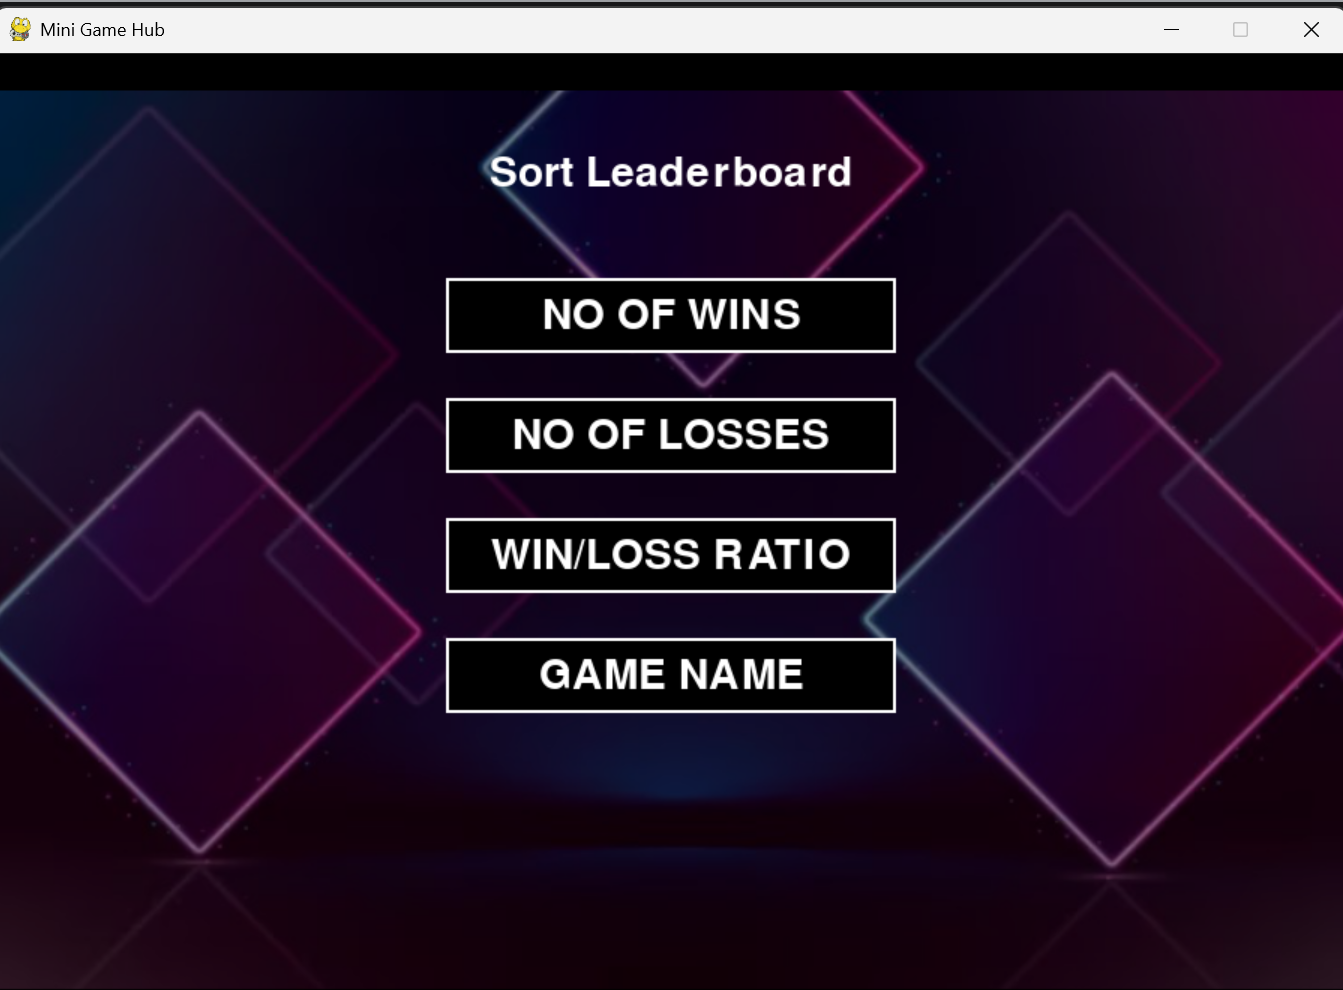
\includegraphics[width=0.8\textwidth]{leaderboard.png}
\caption{Game Interface}
\end{figure}
% ======================================================
\section{Hurdles Faced and Solutions}

\begin{itemize}

\item \textbf{Pygame Window Closing Issue}: Each game used \texttt{pygame.quit()}, which closed the entire application instead of returning to the main menu.  
\textbf{Solution:} Controlled quitting only from main controller (game.py).

\item \textbf{Module Import Errors}: Incorrect import paths caused failures in running games.  
\textbf{Solution:} Fixed folder-based imports using correct package structure.

\item \textbf{Commits on April 11 th are missing} Commits made by Author:Jahnavi-Alaparthi were suddenly missing from the github , while they were showed in github before
\textbf{Solution:} Recommited the code later
. 

\end{itemize}

% ======================================================
\section{What I Would Do If I Had 10 More Hours}

\begin{itemize}

\item Add background music and sound effects.
\item Add animated button effects.
\item Add instruction window before each game.
\item Improve UI transitions and animations.
\item Provide the facility of adding profile  photo (either real or avatar) which is displayed during winning with celebrations.

\end{itemize}

\section{Installation \& Setup}

This section explains the setup process required to run the Mini Game Hub project. The system is designed to work specifically with Python 3.10 and is executed using a Bash script that handles user authentication and launches the main application.

\subsection{Prerequisites}

The following software must be installed before running the project:

\begin{itemize}
    \item Python 3.10 
    \item Bash shell (for execution via \texttt{main.sh})
    \item Pygame library
    \item Matplotlib library
    \item Numpy library
\end{itemize}

\subsection{User Authentication Flow}

The project uses a manual authentication system where the user provides a username and password. These credentials are verified through the shell script and then passed as arguments to the main Python file.

\begin{itemize}
    \item The user enters \textbf{username} and \textbf{password} in the terminal.
    \item \texttt{main.sh} validates and processes the input.
    \item Upon successful validation, credentials are passed to \texttt{game.py} as command-line arguments.
\end{itemize}

\subsection{Project Execution}

The application is launched using the following command:

\begin{verbatim}
bash main.sh
\end{verbatim}

After authentication, the script internally executes:

\begin{verbatim}
python3.10 game.py <username1> <username2>
\end{verbatim}

\subsection{Setup Instructions}

\begin{enumerate}
    \item Ensure Python 3.10 is installed and set as the default Python version.
    \item Install required dependencies:
    \begin{verbatim}
    pip install pygame matplotlib
    \end{verbatim}

    \item Provide execute permissions to shell scripts:
    \begin{verbatim}
    chmod +x main.sh
    \end{verbatim}

    \item Run the project using:
    \begin{verbatim}
    bash main.sh
    \end{verbatim}
\end{enumerate}

\subsection{Important Notes}

\begin{itemize}
    \item The project is strictly compatible with Python 3.10 and may not work correctly on other versions.
    \item All game logic is accessed only after successful authentication through \texttt{main.sh}.
    \item The system relies on command-line arguments to pass authenticated user data into the main game engine.
\end{itemize}


% ======================================================



% ======================================================
\section{Bibliography}

\begin{thebibliography}{99}

\bibitem{pygame} Pygame Documentation. \url{https://www.pygame.org/docs/}
\bibitem{numpy} NumPy Documentation. \url{https://numpy.org/doc/}
\bibitem{matplotlib} Matplotlib Documentation. \url{https://matplotlib.org/}
\bibitem{python} Python Official Documentation. \url{https://docs.python.org/3/}
\bibitem{csv} CSV Module Reference. \url{https://docs.python.org/3/library/csv.html}
\bibitem{sha256} SHA-256 Hashing in Bash. \url{https://man7.org/linux/man-pages/man1/sha256sum.1.html}
\bibitem{classes} Python Classes and Inheritance. \url{https://docs.python.org/3/tutorial/classes.html}
\bibitem{othello} Othello Rules. \url{https://www.worldothello.org/about/about-othello/othello-rules/official-rules/english}
\bibitem{tictactoe} Tic-Tac-Toe Rules. \url{https://en.wikipedia.org/wiki/Tic-tac-toe}
\bibitem{connect4} Connect Four Rules. \url{https://en.wikipedia.org/wiki/Connect_Four}

\end{thebibliography}

\end{document}